%!TEX root = ../../Main.tex
\graphicspath{{Chapters/Opgave2/}}
%-------------------------------------------------------------------------------

\chapter{Design af midlingsfilter}


Vi skal i denne opgave lave et midlingsfilter der kan reducere støjen vi målte i opgave 1. \\
Koden for vores midligsfilter for henholdsvis loaded og unloaded data ses nedenfor. Der er i denne kode taget udgangspunkt i et 10. ordens filter, da N angiver ordenen.

\begin{lstlisting}[frame=single]  % Start your code-block
for i:=maxint to 0 do

N=10;

y=zeros(1,N);
x=zeros(1,N);

unloaded_filtered=zeros(1, length(unloaded)); %Placeholder
loaded_filtered=zeros(1, length(loaded)); %Placeholder

for n=1:length(unloaded)
for k=1:N
if n+k<length(unloaded)
x(k)=unloaded(n+k);
end
end
unloaded_filtered(n)=sum(x)/N;
end

for n=1:length(loaded)
for k=1:N
if n+k<length(loaded)
x(k)=loaded(n+k);
end
end
loaded_filtered(n)=sum(x)/N;
end

\end{lstlisting}

Vi starter med at kigge på et 10. ordens midligsfilter af signalet, i forhold til det ikke filtrede signal i tidsdomænet.\\
\\
\begin{figure}[H]
	\centering
	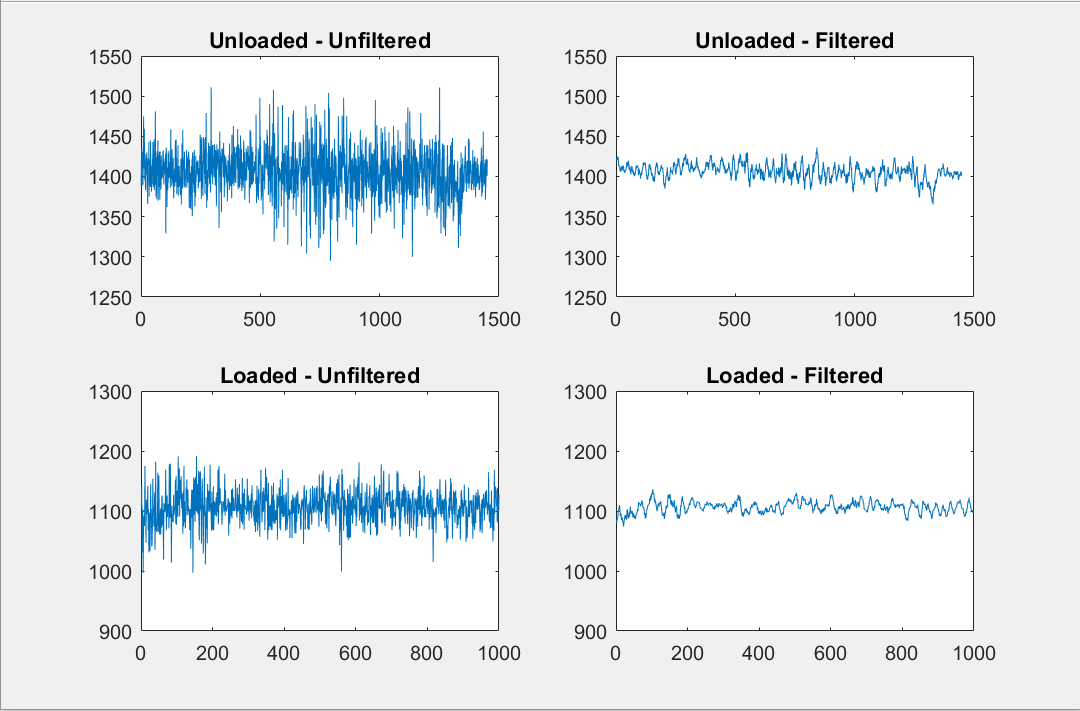
\includegraphics[width = 300pt]{Img/10_ordensfilter.PNG}
	\caption{10. ordens filter vs. ufiltreret signal i tidsdomænet}
	\label{fig:10_ordensfilter}
\end{figure}

Det er meget tydeligt at se reduceringen af støjen før og efter filtreringen. Nu sammenligner vi i tidsdomænet, men denne gang med et 100. ordens midlingsfilter.\\

\begin{figure}[H]
	\centering
	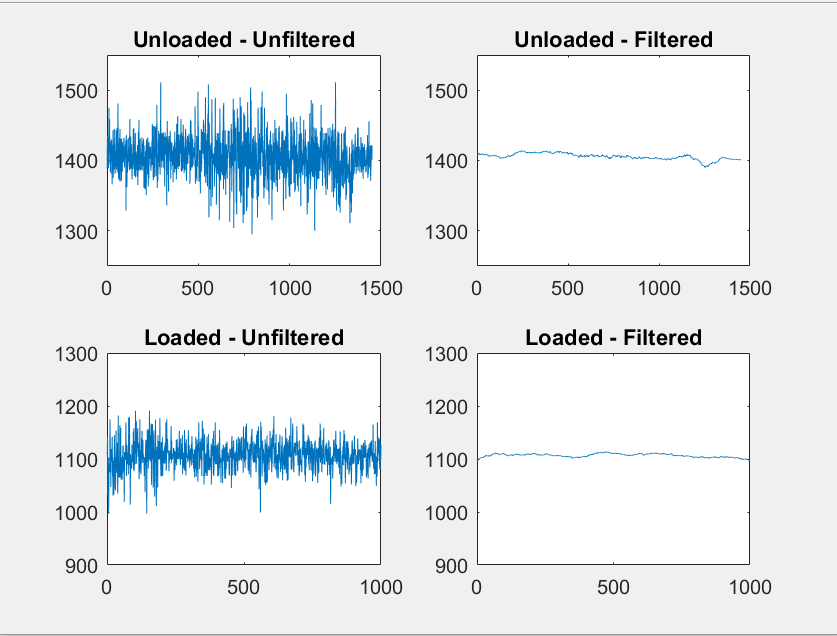
\includegraphics[width = 300pt]{Img/100_ordensfilter.PNG}
	\caption{100. ordens filter vs. ufiltreret signal i tidsdomænet}
	\label{fig:100_ordensfilter}
\end{figure}

Efter signalet har været igennem 100. ordens midlingsfilter, kan man se at støjen stort set er forsvundet i tidsdomænet. \\
Nu vil vi sammenligne histogrammer, varians og støjeffekten. Vi starter med at kigge på histogrammet for 10.ordensfilter kontra det ufiltrerede.
\\\\

\begin{figure}[H]
	\centering
	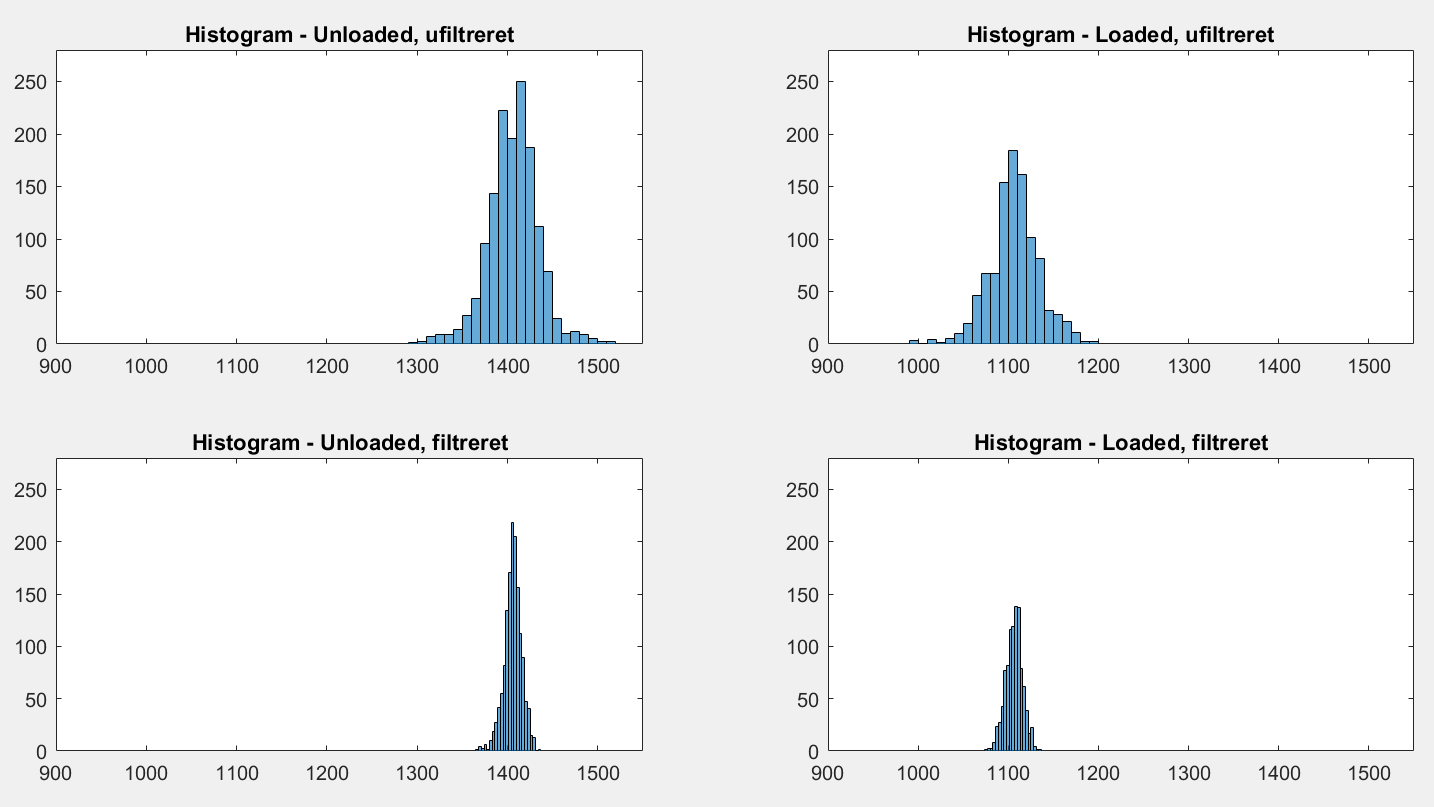
\includegraphics[width = 300pt]{Img/Histogram_10_orden.PNG}
	\caption{10. ordens filter histogram vs. ufiltreret signals histogram}
	\label{fig:Histogram_10_orden}
\end{figure}

På histogrammet er det tydeligt at se, at variansen og standartafvigelsen er blevet betydlig mindre. \\
Variansen for det loaded ufiltrerede signal blev udregnet til 764, det samme signal bare filtreret blev udregnet til 86. Det er næsten en faktor ti mindre, hvilket stemmer meget fint overens med teorien. \\
Standartafvigelsen er gået fra 28 ved det ufiltreret signalt til 9 ved det loadede signal. \\
\\
Nu kigger vi så på histrogrammet for det loaded signal med et 100 ordens filter. \\
\\
\begin{figure}[H]
	\centering
	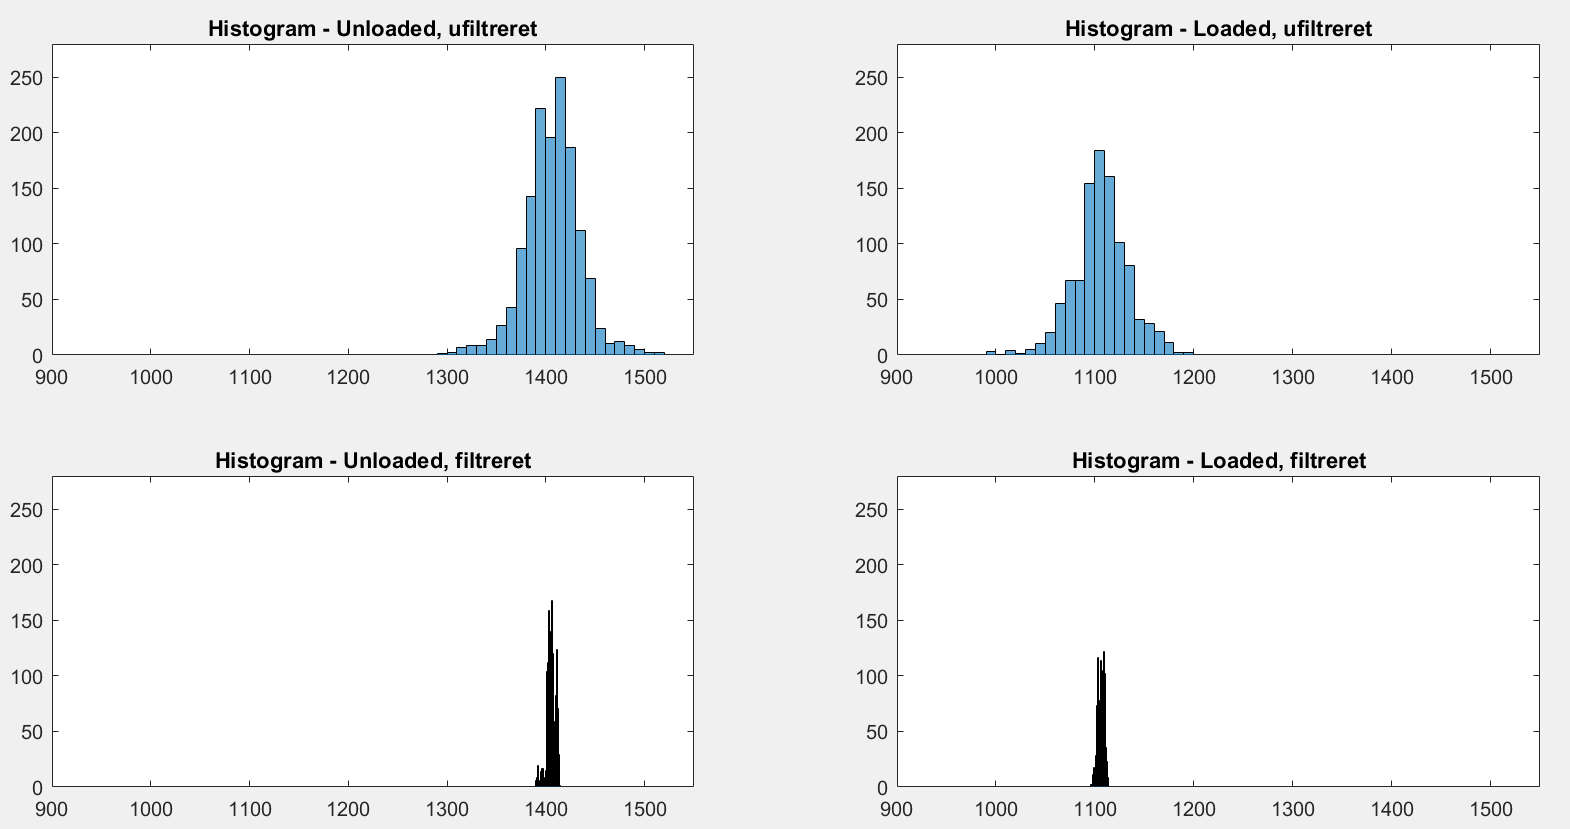
\includegraphics[width = 300pt]{Img/Histogram_100_orden.PNG}
	\caption{100. ordens filter histogram vs. ufiltreret signals histogram}
	\label{fig:Histogram_100_orden}
\end{figure}
På histogrammet er det tydeligt, hvordan variansen og standartafvigelsen for 100. ordens filtereret nu er blevet endnu mindre.
Efter signalt er filtreret med et 100. ordens filter, er variansen for det loadede signal faldet til 11, og standart afvigelsen er faldet til 3. \\
\\
Vi har bestemt os for at have en indsvingningstid på max 100 millisekunder. Så kan den maksimale længe af vores FIR midlingsfilter være på 30 koefficienter, da det giver settle time på ca 30 samples.
\begin{lstlisting}[frame=single]  % Start your code-block
for i:=maxint to 0 do
fs = 300 -> 30 samples = 0.1s = 100ms.
\end{lstlisting}

Herefter dannede vi et eksponentielt midlingsfilter. Vi startede med at eksperimentere med alpha-værdien, for at undersøge hvilket betydning det havde for filteret.\\
\\

\begin{figure}[H]
	\centering
	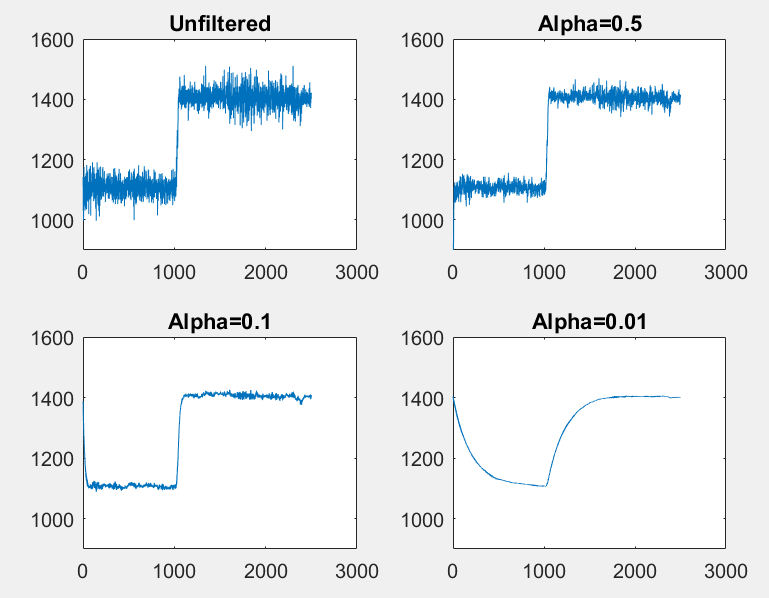
\includegraphics[width = 300pt]{Img/Alpha_variation.PNG}
	\caption{Variation af alpha-værdien}
	\label{fig:Alpha_variation}
\end{figure}

Det kan tydeligt ses hvordan en lavere alpha-værdi reducere støjen. Det bliver dog også tydeligt, når alfa-værdien kommer helt ned på 0.01 at indsvingningstiden bliver større. \\
\\
Til sidst i denne opgave ville vi prøve at sætte alpha-værdien, således vi får samme støj reduktion, som for vores 100. ordens midlingsfilter. 
Fremgangsmåden for dette kan ses i koden nedenfor. \\\\
\\
\\
\\
\\
\\
\\
\\
\\




\begin{lstlisting}[frame=single]  % Start your code-block
for i:=maxint to 0 do

noise_reduction_unloaded_FIR=
var_unloaded_filtered/var_unloaded
noise_reduction_loaded_FIR=var_loaded_filtered/var_loaded

alpha=0.050872;
y_eksp=[0;0];

signal_eksp_filtered=zeros(1,length(vejecelle_data));
for n=1:length(vejecelle_data)
y_eksp(2)=y_eksp(1);
output=alpha*vejecelle_data(n)+(1-alpha)*y_eksp(2);
signal_eksp_filtered(n)=output;
y_eksp(1)=output;
end


\end{lstlisting}

Vi har så efterfølgende sat de to filtre op mod hinanden, som kan ses på billedet nedenfor.\\
\\

\begin{figure}[H]
	\centering
	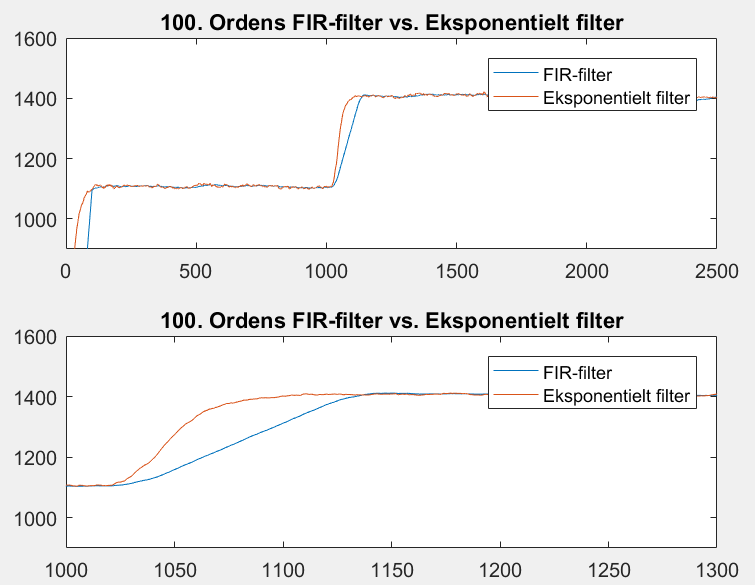
\includegraphics[width = 300pt]{Img/Ekspoentielt_filter.PNG}
	\caption{Ekspoentielt filter vs 100. ordens filter}
	\label{fig:Ekspoentielt_filter}
\end{figure}


Det ses at FIR-filteret lineært tilnærmer sig den ønskede værdi, hvor det eksponentielle filter meget hurtigt stiger til at starte med, hvorefter hældningen bliver mindre. Det skyldes at den nyeste samples får størst vægt, dvs. reagerer
hurtigere på ændringer i input ifht. alm.
midlingsfilter. Så umiddelbart ser det eksponentielle filter ud til
at være mere responsivt.